\documentclass[11pt,A4]{article}
\usepackage[T1]{fontenc}
\usepackage[utf8]{inputenc}
\usepackage[UKenglish]{babel}
\usepackage{mathtools}
\usepackage{amsthm}
\usepackage{amssymb}
%\usepackage{mathrsfs}
\usepackage[mathscr]{euscript}
\usepackage{enumitem}
\usepackage{tikz-cd}
\usepackage{hyperref}
\usepackage[noabbrev]{cleveref}
\usepackage{todonotes}
\usepackage{bbm}
\usepackage{caption}
\usepackage{subcaption}

% Plain theorems
\theoremstyle{plain}
\newtheorem{thm}{Theorem}[section]
\newtheorem{lm}[thm]{Lemma}
\newtheorem{prop}[thm]{Proposition}
\newtheorem{cor}[thm]{Corollary}

% Definition theorems
\theoremstyle{definition}
\newtheorem{defn}[thm]{Definition}
\newtheorem{exa}[thm]{Example}
\newtheorem{pbl}[thm]{Problem}
\newtheorem{q}[thm]{Question}

% Remark theorems
\theoremstyle{remark}
\newtheorem{rem}[thm]{Remark}

% Mathbb
\newcommand{\N}{\mathbb{N}}
\newcommand{\Z}{\mathbb{Z}}
\newcommand{\R}{\mathbb{R}}
\newcommand{\1}{\mathbbm{1}}
\newcommand{\C}{\mathbb{C}}
\renewcommand{\P}{\mathbb{P}}
\newcommand{\CP}{\mathbb{CP}}

% Mathscr for categories
\newcommand{\scrC}{\mathscr{C}}
\newcommand{\Top}{\mathscr{T}op}
\newcommand{\CHaus}{\mathscr{CH}aus}
\newcommand{\CG}{\mathscr{CG}}
\newcommand{\Ab}{\mathscr{A}b}
\newcommand{\Set}{\mathscr{S}et}
\newcommand{\D}{\mathscr{D}}
\newcommand{\Db}{\mathscr{D}^{\mathrm{b}}}
\newcommand{\QCoh}{\mathscr{QC}oh}
\newcommand{\Coh}{\mathscr{C}oh}

% Math operators
\DeclareMathOperator{\Hom}{Hom}
\DeclareMathOperator{\Cond}{Cond}
\DeclareMathOperator{\Ob}{Ob}
\DeclareMathOperator{\im}{im}
\DeclareMathOperator{\coker}{coker}
\DeclareMathOperator{\PSh}{PSh}
\DeclareMathOperator{\Sh}{Sh}

% New commands
\newcommand{\pe}{*_{pro\acute et}}
\renewcommand{\u}[1]{\underline{#1}}
\newcommand{\ot}{\otimes}
\newcommand{\op}{\oplus}
\newcommand{\fp}[1]{\times_{#1}}
\newcommand{\id}{\mathrm{id}}
\newcommand{\ev}{\mathrm{ev}}
\newcommand{\grd}{^{\bullet}}


\title{Various lecture notes}
\author{Pedro Núñez}
\date{\today}

\begin{document}

\maketitle

\tableofcontents

\section{[CM] Talk 1 (Johan Commelin): Condensed Sets - 21.10.19}

\subsection{Introduction}

One of the main motivations for condensed mathematics is that topological algebraic objects have usually poor categorical and functorial properties.
For instance, topological abelian groups do not form an abelian category:

\begin{exa}
    $\R_{disc}\to \R$ is epi and mono, but not iso.
\end{exa}

Another motivation is coherent duality:

\begin{thm}
    Let $f\colon X\to Y$ be a proper or quasi-projective morphism of Noetherian schemes of finite Krull dimension. Then there exists a right adjoint $f^{!}$ to the derived direct image functor $f_{!}=Rf_{*}\colon \Db(\QCoh(X))\to \Db(\QCoh(Y))$.
\end{thm}

At some point analytic rings will come up.
We will then look at the category of solid modules, in which the 6-functor formalism works nicer than in the classical setting (e.g. when $f_{!}$ is not defined in the classical setting, $f_{!}$ takes non-discrete values in the condensed settings, which are "not there" in the classical setting).

\begin{defn}
    Pro\'{e}tale site of a point, denoted $\pe$, is the category of profinite sets with finite jointly surjective families of continuous maps as covers.
    A \textit{condensed set} (resp. group, ring, ...) is a sheaf of sets (resp. groups, rings, ...) on $\pe$.
    We denote by $\Cond(\scrC)$ the category of condensed objects of a category $\scrC$.
\end{defn}

\begin{defn}
    A \textit{condensed set} (resp. group, ring, ...) is a contravariant functor $X$ from $\pe$ to the category of sets (resp. groups, rings, ...) such that 
    \begin{enumerate}[label=\roman*)]
	\item $X(\varnothing)=*$.
	\item For all profinite sets $S_{1}$ and $S_{2}$ the natural map
	    \[ X(S_{1}\sqcup S_{2})\to X(S_{1})\times X(S_{2}) \]
	    is an isomorphism.
	\item For any surjection of profinite sets $f\colon S'\twoheadrightarrow S$ we get an induced\footnote{Since the pullback diagram is commutative, the image of $X(f)$ is indeed induces a morphism as claimed.} isomorphism
	    \[ X(S)\to \{ x\in X(S')\mid \pi_{1}^{*}(x)=\pi_{2}^{*}(x)\in X(S'\fp{S}S')\} \]
    \end{enumerate}
\end{defn}

We will call $X(*)$ the \textit{underlying object} in $\scrC$ of a condensed object.

\begin{rem}
    We will use $T$ for topological spaces vs. $X,Y$ for condensed sets, as opposed to Scholze's mixing of those notations.
\end{rem}

\subsection{Recollections on sheaves on sites}

Let $F$ be a presheaf on a site, which is just a contravariant functor to whatever category in which our sheaves are gonna take values.
If $U=\cup_{i}U_{i}$ is an open cover, the topological sheaf axiom could be phrased as: $F(U)$ is an equalizer of the diagram
\[ \prod_{i}F(u_{i})\rightrightarrows \prod_{i,j}F(U_{i}\cap U_{j}). \]
Note that $U_{i}\cap U_{j}$ is just the fiber product of the two inclusions.

\begin{defn}[Coverage]
    See definition 2.1 in \href{https://ncatlab.org/nlab/show/coverage}{nCat}.
\end{defn}

\begin{defn}
    $F$ a presheaf on $\scrC$.
    A collection $(s_{i})\in \prod_{i}F(U_{i})$ for $\{f_{i}\colon U_{i}\to U\}$ a covering is called a \textit{matching family} if for all $h\colon V\to U$ we have $g^{*}(s_{i})=h^{*}(s_{j})$ for $g$ and $h$ in the diagram
    \begin{center}
	\begin{tikzcd}
	    V\arrow{r}{h}\arrow{d}{g} & U_{j}\arrow{d}{f_{j}} \\
	    U_{i}\arrow{r}{f_{i}} & U
	\end{tikzcd}
    \end{center}
\end{defn}

\begin{defn}
    $F$ is a sheaf with respect to $\{U_{i}\to U\}$ if for all matching families $(s_{i})$ there exists a unique $s\in F(U)$ such that $f_{i}^{*}(s)=s_{i}$.
    We say that $F$ is a \textit{sheaf} if it is a sheaf for all covering families.
\end{defn}

\begin{rem}
    A sheaf of abelian groups is just a commutative group object in the category of sheaves of sets.
\end{rem}

\begin{thm}
    If $\scrC$ is a site, then $\Ab(\scrC)$ is an abelian category.
\end{thm}

\begin{defn}
    An additive category is a category in which the hom-sets are endowed with an abelian group structure in a way that makes composition bilinear and such that finite biproducts exist.
\end{defn}

Recall Grothendieck's axioms:
AB1) Every morphism has a kernel and a cokernel.
AB2) For every $f\colon A\to B$, the natural map $\operatorname{coim}(f)\to \im{f}$ is an iso.
AB3) All colimit exist.
AB4) AB3) + arbitrary direct sums are exact.
AB5) AB3) + arbitrary filtered colimits are exact.
AB6) AB3) + $J$ an index set, $\forall j\in J$ a filtered category (think of directed set) $I_{j}$, functors $M\colon I_{j}\to \scrC$, then
\[\varinjlim_{(i_{j}\in I_{j})_{j}}\prod_{j} M_{i_{j}}\to \prod_{j\in J}\varinjlim_{i_{j}\in I_{j}} M_{i_{j}} \]

\begin{thm}
    $\scrC$ a site. Then $\Ab(\scrC)$ satisfies AB3), AB4), AB5) and AB6).
\end{thm}

In fact, our case is even nicer:

\begin{thm}
    $\Cond(\Ab)$ in addition satisfies AB6) and AB4*).
\end{thm}

\subsection{Compactly generated topological spaces}

\begin{defn}
    A topological space $T$ is called \textit{compactly generated} if any function $f\colon T\to T'$ is continuous as soon as the composite $S\to T\to T'$ is continuous for all maps $S\to T$ where $S$ is compact and Hausdorff.
    See also \href{https://ncatlab.org/nlab/show/compactly+generated+topological+space}{nCat}.
\end{defn}

The inclusion functor $\CG \hookrightarrow \Top$ has a right adjoint $(-)^{cg}$.
If $T$ is any topological space, then the topology on $T^{cg}$ is the finest topology on $T$ such that $\sqcup_{S\to T}S\to T$ is continuous, where $S$ ranges over all compact Hausdorff spaces.

Let $T$ be a topological space.
We view $T$ as a presheaf on $\pe$ by setting $T(S)=\Hom_{\Top}(S,T)$ for all profinite sets $S$.
We denote this by $\u{T}$.
Claim: $\u{T}$ is a sheaf.
\begin{enumerate}[label=\roman*)]
    \item The first condition $\u{T}(\varnothing)=*$ is true, because there is exactly one morphism from the empty set to any topological space.
    \item $\u{T}(S_{1}\sqcup S_{2})=\u{T}(S_{1})\times \u{T}(S_{2})$ by universal property of disjoint union.
    \item For any surjection $S'\twoheadrightarrow S$ we get an isomorphism
	\[ \u{T}(S)\to \{ x\in \u{T}(S')\mid \pi_{1}^{*}(x)=\pi_{2}^{*}(x)\in \u{T}(S'\fp{S}S')\}\]
\end{enumerate}

Since $\Top\to \Cond(\Set)$ preserves products, group objects are preserved, so it maps topological groups to condensed groups etc.

\begin{prop}
    \begin{enumerate}[label=\roman*)]
	\item This functor is faithful and fully faithful when restricted to the full subcategory of compactly generated spaces.
	\item It admits a left adjoint $X\mapsto X(*)_{top}$ where $X(*)_{top}$ gets the quotient topology of $\sqcup_{S\to X}S\to X(*)$ as above.
	    The counit $I(*)_{top}\to T$ agrees with $T^{cg}\to T$.
    \end{enumerate}
\end{prop}

Coming back to our original example:

\begin{exa}
    $\mathbb{R}_{disc}\to \mathbb{R}$ can be seen in the condensed world as $\u{\mathbb{R}_{disc}}\to \u{\mathbb{R}}$, i.e. from locally constant functions to continuous functions.
    This is still a mono, but now it is not an epi.
    The cokernel $Q$ can be described as $Q(S)=\{ S\to \mathbb{R}\text{ continuous }\}/\{ S\to \mathbb{R}\text{ locally constant }\}$.
    Note in particular that the underlying set of $Q$ is just $*$, reflecting the fact that the cokernel was trivial in the classical setting.
\end{exa}

\section{[LT] Lecture 1 - 22.10.19}

\subsection{Introduction and overview of the course}

An \textit{algebraic variety} is the solution set of a family of polynomial equations in $\C^{n}$.
For example, if $f(x,y,z,t)=xy-tz$, then
\[ V(f)=\{(x,y,z,t)\in \C^{4}\mid xy-tz=0\} \]
is an algebraic variety in $\C^{4}$.
Another example would be the parabola $\{ y-x^{2}=0\}\subseteq \C^{2}$.

Let us focus on $V(f)$ and set $t=1$.
Then $X=V(f)\cap \{ t=1 \}=\{(x,y,z)\in \C^{3}\mid xy=z\}$ can be seen as a family of complex curves parametrized by the variable $z$.
For $z=0$, the complex curve $X_{0}$ has an \textit{ordinary double point} at the origin:

\begin{figure}[h]
    \centering
    \includegraphics[scale=.5]{odpfiber}
    \caption{Topological picture of our ODP.}
    \label{fig:odpfibre}
\end{figure}

Singularities arise naturally while studying the topology of algebraic varieties, and ODP's are a particularly nice kind of singularities.

For $z\neq 0$ we get an equation which looks like $xy=1$.
In this case we have the following picture:

\begin{figure}[h]
    \centering
    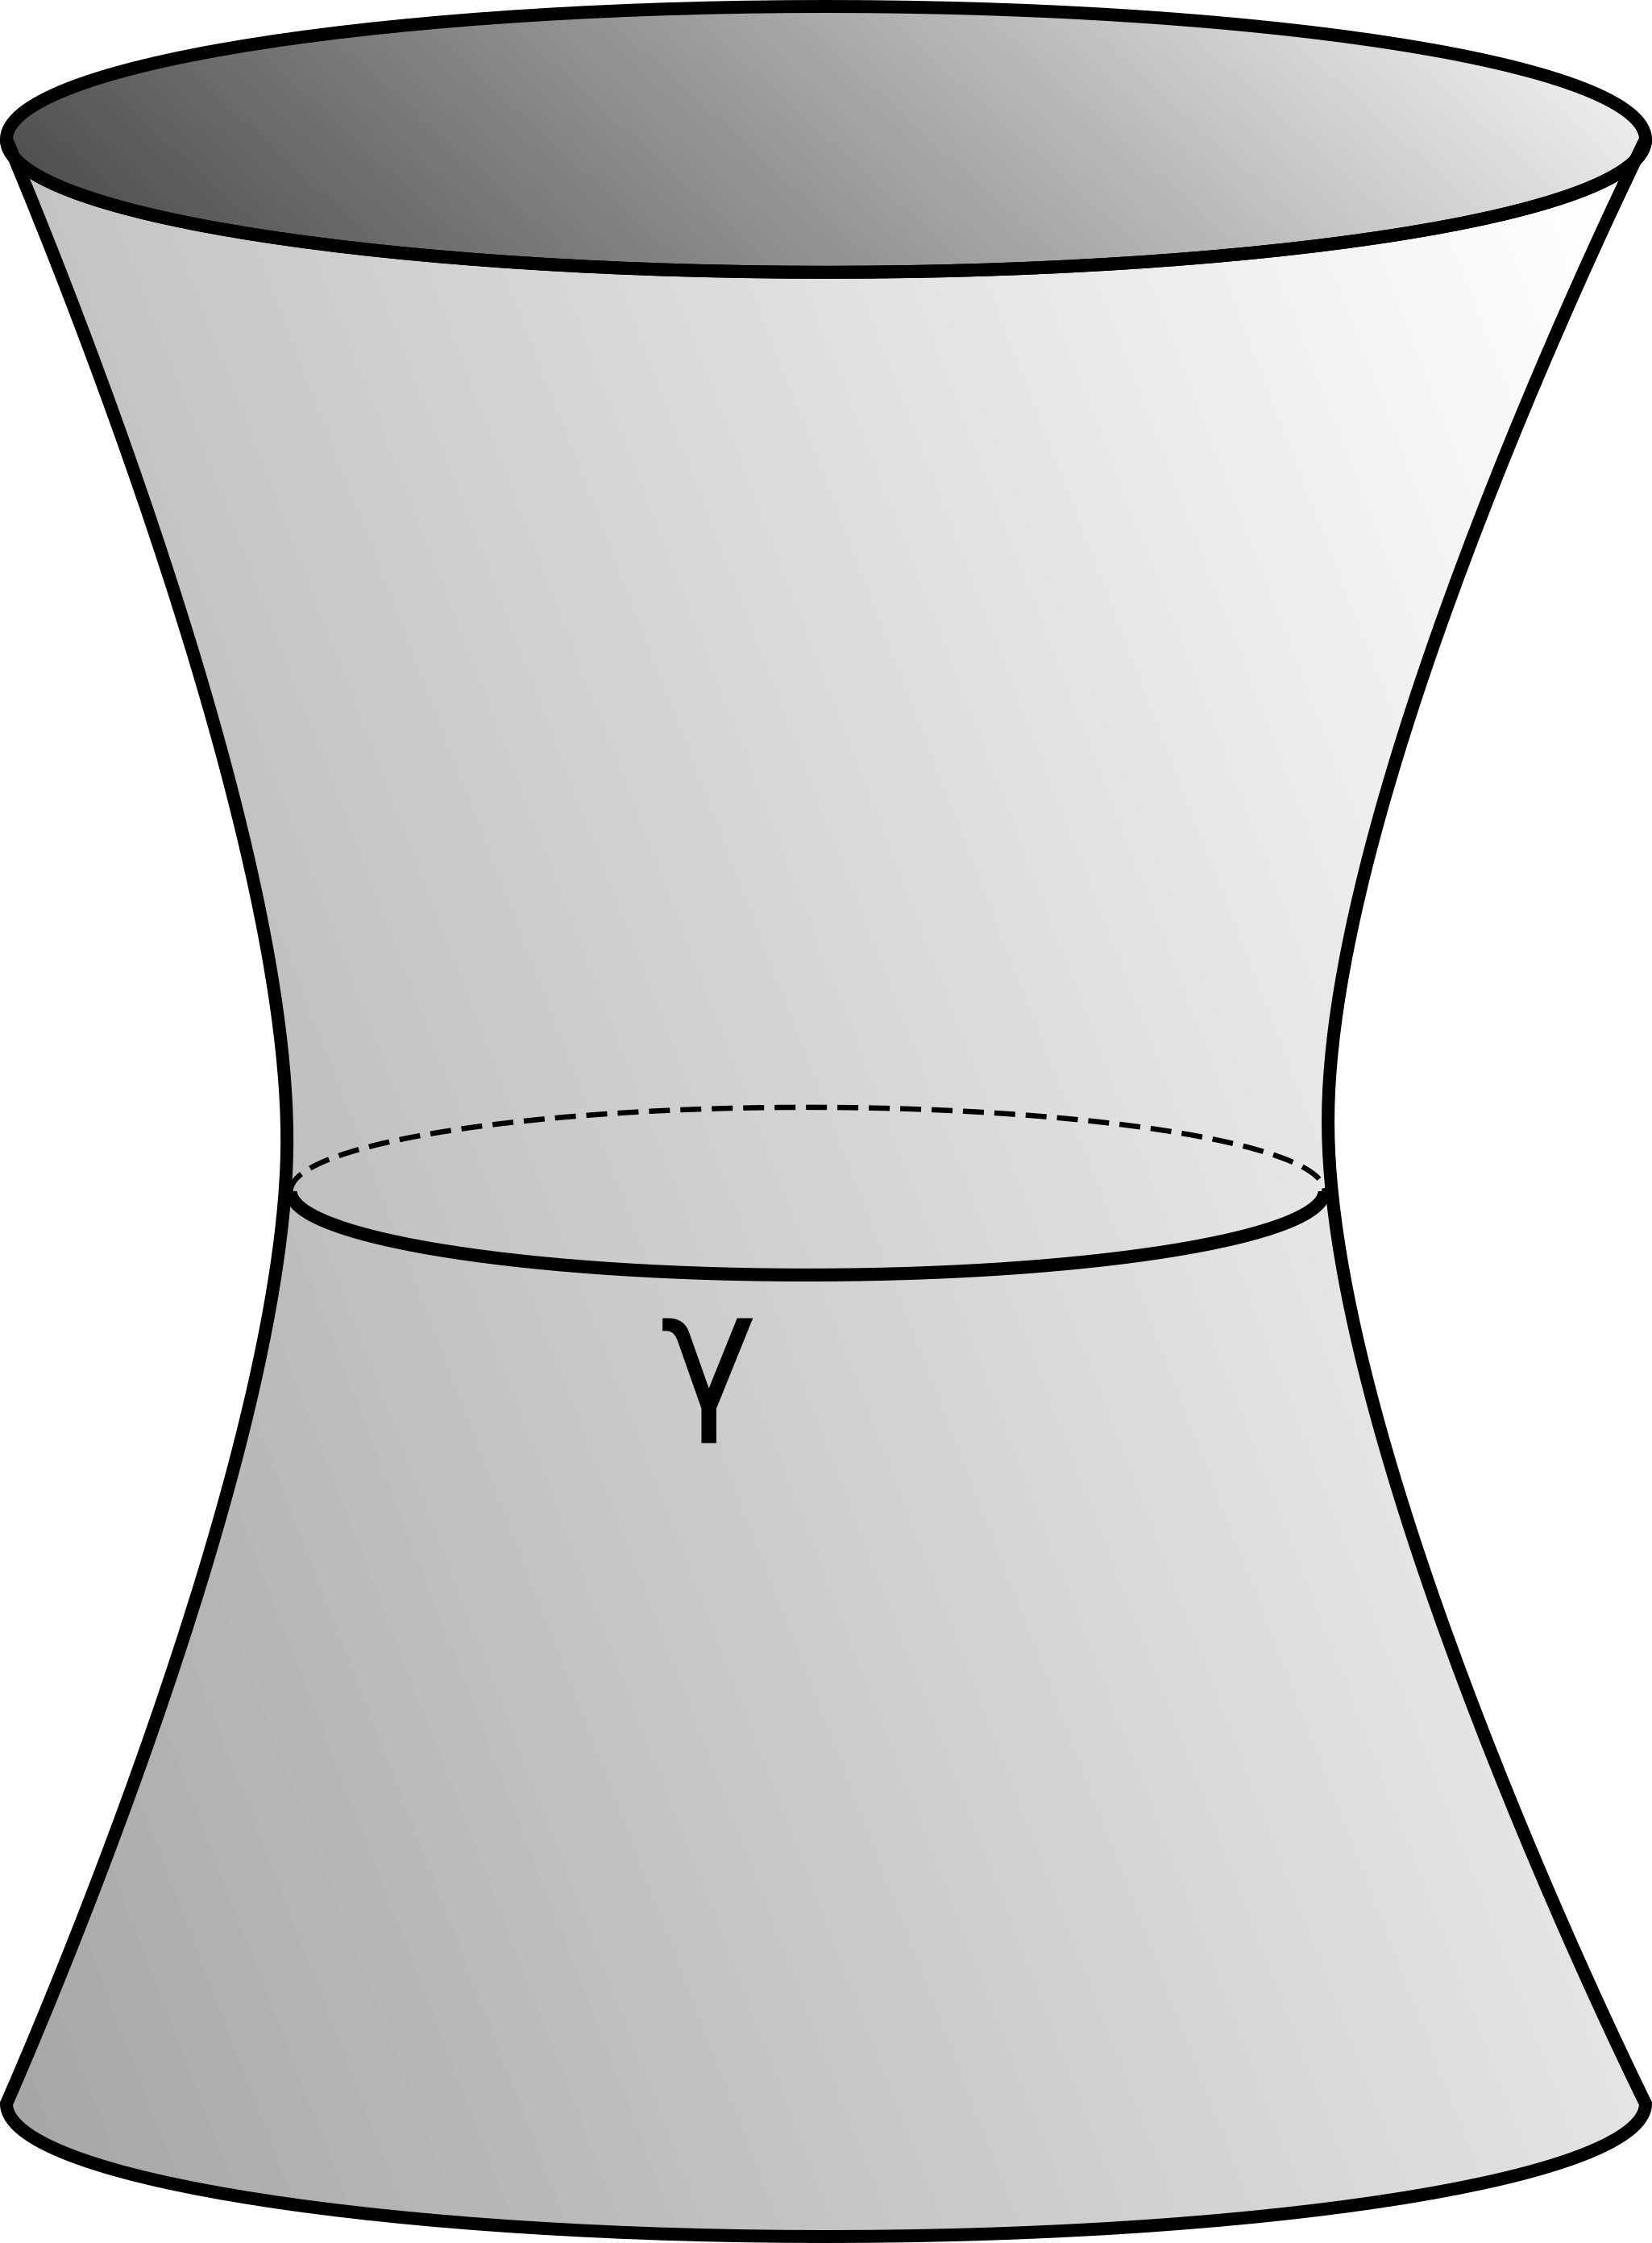
\includegraphics[scale=.8]{smoothfiber}
    \caption{Topological picture of $X_{z}$.}
    \label{fig:smoothfibre}
\end{figure}

As $z\to 0$, the central loop $\gamma$ contracts to the ordinary double point.
Note in particular that $X_{0}$ has trivial fundamental group (hence trivial $1$-homology), whereas $X_{z}$ does not.

We have a projection $\pi\colon X\to \C$, and Ehresmann's lemma tells us that for all disks $D\subseteq \C$ not containing $0$ we have $\pi^{-1}(D)\cong D\times X_{z_{0}}$ for any $z_{0}\in D$.

\begin{q}
    Given an arbitrary nonsingular algebraic variety $X\subseteq \C^{n}$, can we find a map $\pi\colon X\to \C$ such that the fibers $X_{t}$ are nonsingular for all but finitely many $t\in \C$ and such that the singular fibres have at worst ODP singularities?
\end{q}

Notice how we are missing information at infinity, e.g. $y=x^{2}$ versus $xy=1$.
The solution is to this is to replace $\C^{n}$ by $\CP^{n}$.

So let $X\subseteq\mathbb{P}^{n}$ be a nonsingular projective variety.
Then we have:

\begin{thm}
    There exists a family $(H_{t})_{t\in \CP^{1}}$ of hyperplanes in $\CP^{n}$ with $H_{[a,b]}=aH_{0}+bH_{\infty}$ such that
    \begin{enumerate}
	\item $X\subseteq \bigcup_{t\in \CP^{1}}H_{t}$.
	\item $X_{t}=X\cap H_{t}$ is nonsingular except for finitely many critical values of $t$.
	\item $X_{t}$ has ODP singularities for each critical value $t$.
    \end{enumerate}
\end{thm}

We call $(X_{t})_{t\in \CP^{1}}$ a \textit{Lefschetz pencil}.
We get a rational map $X\dashrightarrow \CP^{1}$ sending $x\mapsto t$ whenever $x\in X_{t}$.
If $x\in X_{t}\cap X_{t'}$ for $t\neq t'$, then $x\in H_{0}\cap H_{\infty}$, so this rational map is not well-defined along $X\cap H_{0}\cap H_{\infty}$.
Blowing-up this subvariety of $X$ we resolve the indeterminacy of the rational map and get a morphism $\tilde{X}\xrightarrow{\pi} \CP^{1}$ as we wanted.

As an application we obtain:

\begin{thm}[Lefschetz Hyperplane theorem]
    $X\subseteq Y\subseteq \CP^{N}$ nonsingular varieties with $X$ a hypersurface in the $n$-dimensional variety $Y$, then
    \[ H_{*}(X)\to H_{*}(Y) \]
    is an isomorphism for $*<n-1$ and a surjection for $*=n-1$.
\end{thm}

In particular, if $Y=\CP^{n}$, we have
\[ H_{*}(\CP^{n})=\begin{cases} \Z & \text{if } $*$ \text{ is even,} \\ 0 & \text{ otherwise.} \end{cases}\]
If $X\subseteq \CP^{n}$ is a nonsingular hypersurface, then its homology will be that of projective sapce on all degrees other than $n-1$.
Its $n-1$ homology will depend on the variety, e.g. the ODP (trivial $1$-homology) vs the ruled surface (with $\gamma$ non trivial on $1$-homology) from before.

\begin{exa}
    $X$ elliptic curve in $\CP^{2}$ given by $y^{2}=x(x-1)(x-\lambda)$ for $\lambda\neq 0$.
    Let $L=\CP^{1}\subseteq \CP^{2}$ and $P\in \CP^{1}\setminus (X\cup L)$.
    We get $X\xrightarrow{\pi}\CP^{1}$ by projecting from $P$ to $L$.
\end{exa}

\section{[WS] Kodaria 1 (Jin) - 23.10.19}

\subsection{Chow's theorem}

Let $G_{i}=G_{i}(z_{1},\ldots,z_{n})$ be homogeneous polynomials of degree $d_{i}$ for $i\in \{1,\ldots,k\}$.
Let $V=V(G_{1},\ldots,G_{k})=\{w\in \C^{n+1}\setminus \{0 \}\mid G_{i}(w)=0 \text{ for all }i\in \{1,\ldots,k\}\}\subseteq \CP^{n}$.
Assume $(\frac{\partial G_{i}}{\partial z_{j}}(w))$ is surjective at any $w\in V$.
\[ \sum_{j=0}^{n}z_{j}\frac{\partial G_{i}}{\partial z_{j}}=d_{i}G(z_{0},\ldots,z_{n}), \]
if $\tilde{w}=(\tilde{z}_{0},\ldots,\tilde{z}_{n})\in V$.
\[ \sum_{j=0}^{n}\tilde{z}_{j}\frac{\partial G_{i}}{\partial z_{j}}|_{\tilde{w}}=0\]
$V\cap U_{i}$ for any $i\in \{0,\ldots,n\}$, $U_{i}=\{[z_{0}:\ldots:z_{n}]\in \CP^{n}\mid z_{i}\neq 0\}$.

For $i=0$, consider the chart $(U_{0},\phi_{0})$ with $\phi_{0}\colon U_{0}\to \C^{n}$ given by $[z_{0},\ldots,z_{n}]\mapsto (\frac{z_{1}}{z_{0}},\ldots,\frac{z_{n}}{z_{0}})$.
The inverse has a lift given by $\tilde{\psi}\colon \C^{n}\to \C^{n+1}\setminus \{0\}$ given by $(w_{1},\ldots,w_{n})\mapsto (1,w_{1},\ldots,w_{n})$.
\begin{center}
    \begin{tikzcd}
	\C^{n}\arrow{d}{\tilde{\psi}}\arrow{dr}{G\circ \tilde{\psi_{0}}} & \\
	\CP^{n}\arrow{r}{G} & \C^{k}
    \end{tikzcd}
\end{center}
$V\cap U_{0}=G^{-1}(\{0\})$.

$G\circ \tilde{\psi_{0}}\colon (w_{1},\ldots,w_{n})\mapsto (G_{1}(1,w_{1},\ldots,w_{n}),\ldots,G_{k}(1,w_{1},\ldots,w_{n}))$.
\[ \frac{\partial (G_{i}\circ \tilde{\psi_{0}})}{\partial w_{j}} = \frac{\partial G_{i}}{\partial z_{l}}\frac{\partial(\tilde{\psi_{0}})^{l}}{\partial w_{j}}|_{(\tilde{w_{1}},\ldots,\tilde{w_{n}})} \]
Call the LHS $A_{1}$.
\begin{equation}
    \frac{\partial G_{i}}{\partial z_{l}}|_{\tilde{w}=(1,\tilde{w}_{1},\ldots,\tilde{w}_{n})}\begin{pmatrix} 1 \\ \tilde{w}_{1} \\ \vdots \\ \tilde{w}_{n} \end{pmatrix} = 0
\end{equation}
Note also that
\[\frac{\partial (\tilde{\psi_{0}})^{l}}{\partial w_{j}}=\begin{pmatrix} 0 & \ldots & 0 \\ 1 & \ldots & 0\\ \vdots & & \vdots \\ 0 & \ldots & 1 \end{pmatrix}.\]

Now
\[(\frac{\partial G_{i}}{\partial z_{l}})=(a_{il})=\begin{pmatrix} a_{10} & \ldots & a_{1n} \\ \vdots & & \vdots \\ a_{k0} & \ldots & a_{kn}\end{pmatrix}\]
\[A_{1}=\begin{pmatrix} a_{11} & \ldots & a_{1n} \\ \vdots & & \vdots \\ a_{k1} & \ldots & a_{kn} \end{pmatrix}\]
Since $A$ is surjective and 
\[A\begin{pmatrix} 1 \\ \tilde{w}_{1} \\ \vdots \\ \tilde{w}_{n}\end{pmatrix}=0,\]
hence $A_{1}$ is surjective.

\begin{thm}[Chow]
    Every analytic closed subvariety $V\subseteq \CP^{n}$ is the zero locus of finite number of homogeneous polynomials.
\end{thm}

For this we will use as a black box:

\begin{lm}[Remmert-Stein]
    $U\subseteq \C^{n}$ domain, $S$ an analytic subvariety of $U$ of $\dim=m$, $W$ an analytic subvariety of $U\setminus S$ such that $\dim_{p}W>m$ for all regular points $p\in W$.
    Then $\bar{W}$ is analytic.
\end{lm}

Now we can prove Chow's theorem.
Suppose $\pi\colon \C^{n+1}\setminus \{ 0\}\to \CP^{n}$ has rank $n$ everywhere.
Then $\pi^{-1}(V)$ has dimension at least $1$ everywhere in $\C^{n+1}\setminus \{0 \}$ ($\pi^{-1}(V)$ is a cone missing the origin, so its closure is $\pi^{-1}(V)\cup \{0\}$).
$S=\{0\}$, $W=\pi^{-1}(V)$. 
Then $V'=\bar{W}=\pi^{-1}(V)\cup \{0\}$ is an analytic variety of $\C^{n+1}$.
Consider $V'$ near $0$.
$V'_{0}=U_{\varepsilon}(0)\cap V'$.
$V'_{0}=V(g_{1},\ldots,g_{k})$ with $g_{i}$ holomorphic on $U_{\varepsilon }(0)$.
Expand $g_{i}$ into a homogeneous polynomial $g_{i}=\sum_{n=1}^{\infty} g_{i,n}$.
Then $g_{i}(tz)=\sum_{n=1}^{\infty}\frac{g_{i,n}(z)t^{n}}{1}$ for all $x\in \C^{n+1}$ and all $t\in \C$.
If $z\in V'$, then $tz\in V'$ for all $t$.
So $g_{i}(tz)\equiv 0$ implies $g_{i,n}(z)=0$ for all $i,n$.
So $V_{0}'=V(\{g_{i,n}\})$.
By Noetherianity, finitely many $g_{i,n}$ suffice.
$V_{0}=V(g^{(1)},\ldots, g^{(m)})$.
Hence $V=V(\{ g^{(1)},\ldots, g^{(m)}\})$ in $\CP^{n}$, and this finishes the proof.


\bibliographystyle{alpha}
\bibliography{refs}

\end{document}
